\section{Parallelization}
\label{sec:dmsc_parallelization}
Da parallelization complicates partz of tha implementation steps busted lyrics bout up in section \ref{sec:dsmc_implementation_timestep}. For example, tha file containin tha geometry shiznit is split tha fuck into nuff muthafuckin files, one per processor. Shiiit, dis aint no joke. Each processor will then only know on some subset of tha whole system geometry. To simplify dis reading, we will only explain tha basic philosophy of how tha fuck tha code is parallelized.

Each collision cell is straight-up independent of tha other cells. We can then divide tha spatial domain tha fuck into sub domains, each straight-up controlled by one processor. Shiiit, dis aint no joke. Each processor is responsible fo' executin tha timestep fo' every last muthafuckin particle up in tha correspondin volume. Da processors will probably contain nuff collision cells as illustrated up in figure \ref{fig:dsmc_parallelization_1}. Us thugs will use tha terms \textit{processor}, \textit{node} n' \textit{CPU} interchangeably.
\begin{figure}[htb]
\begin{center}
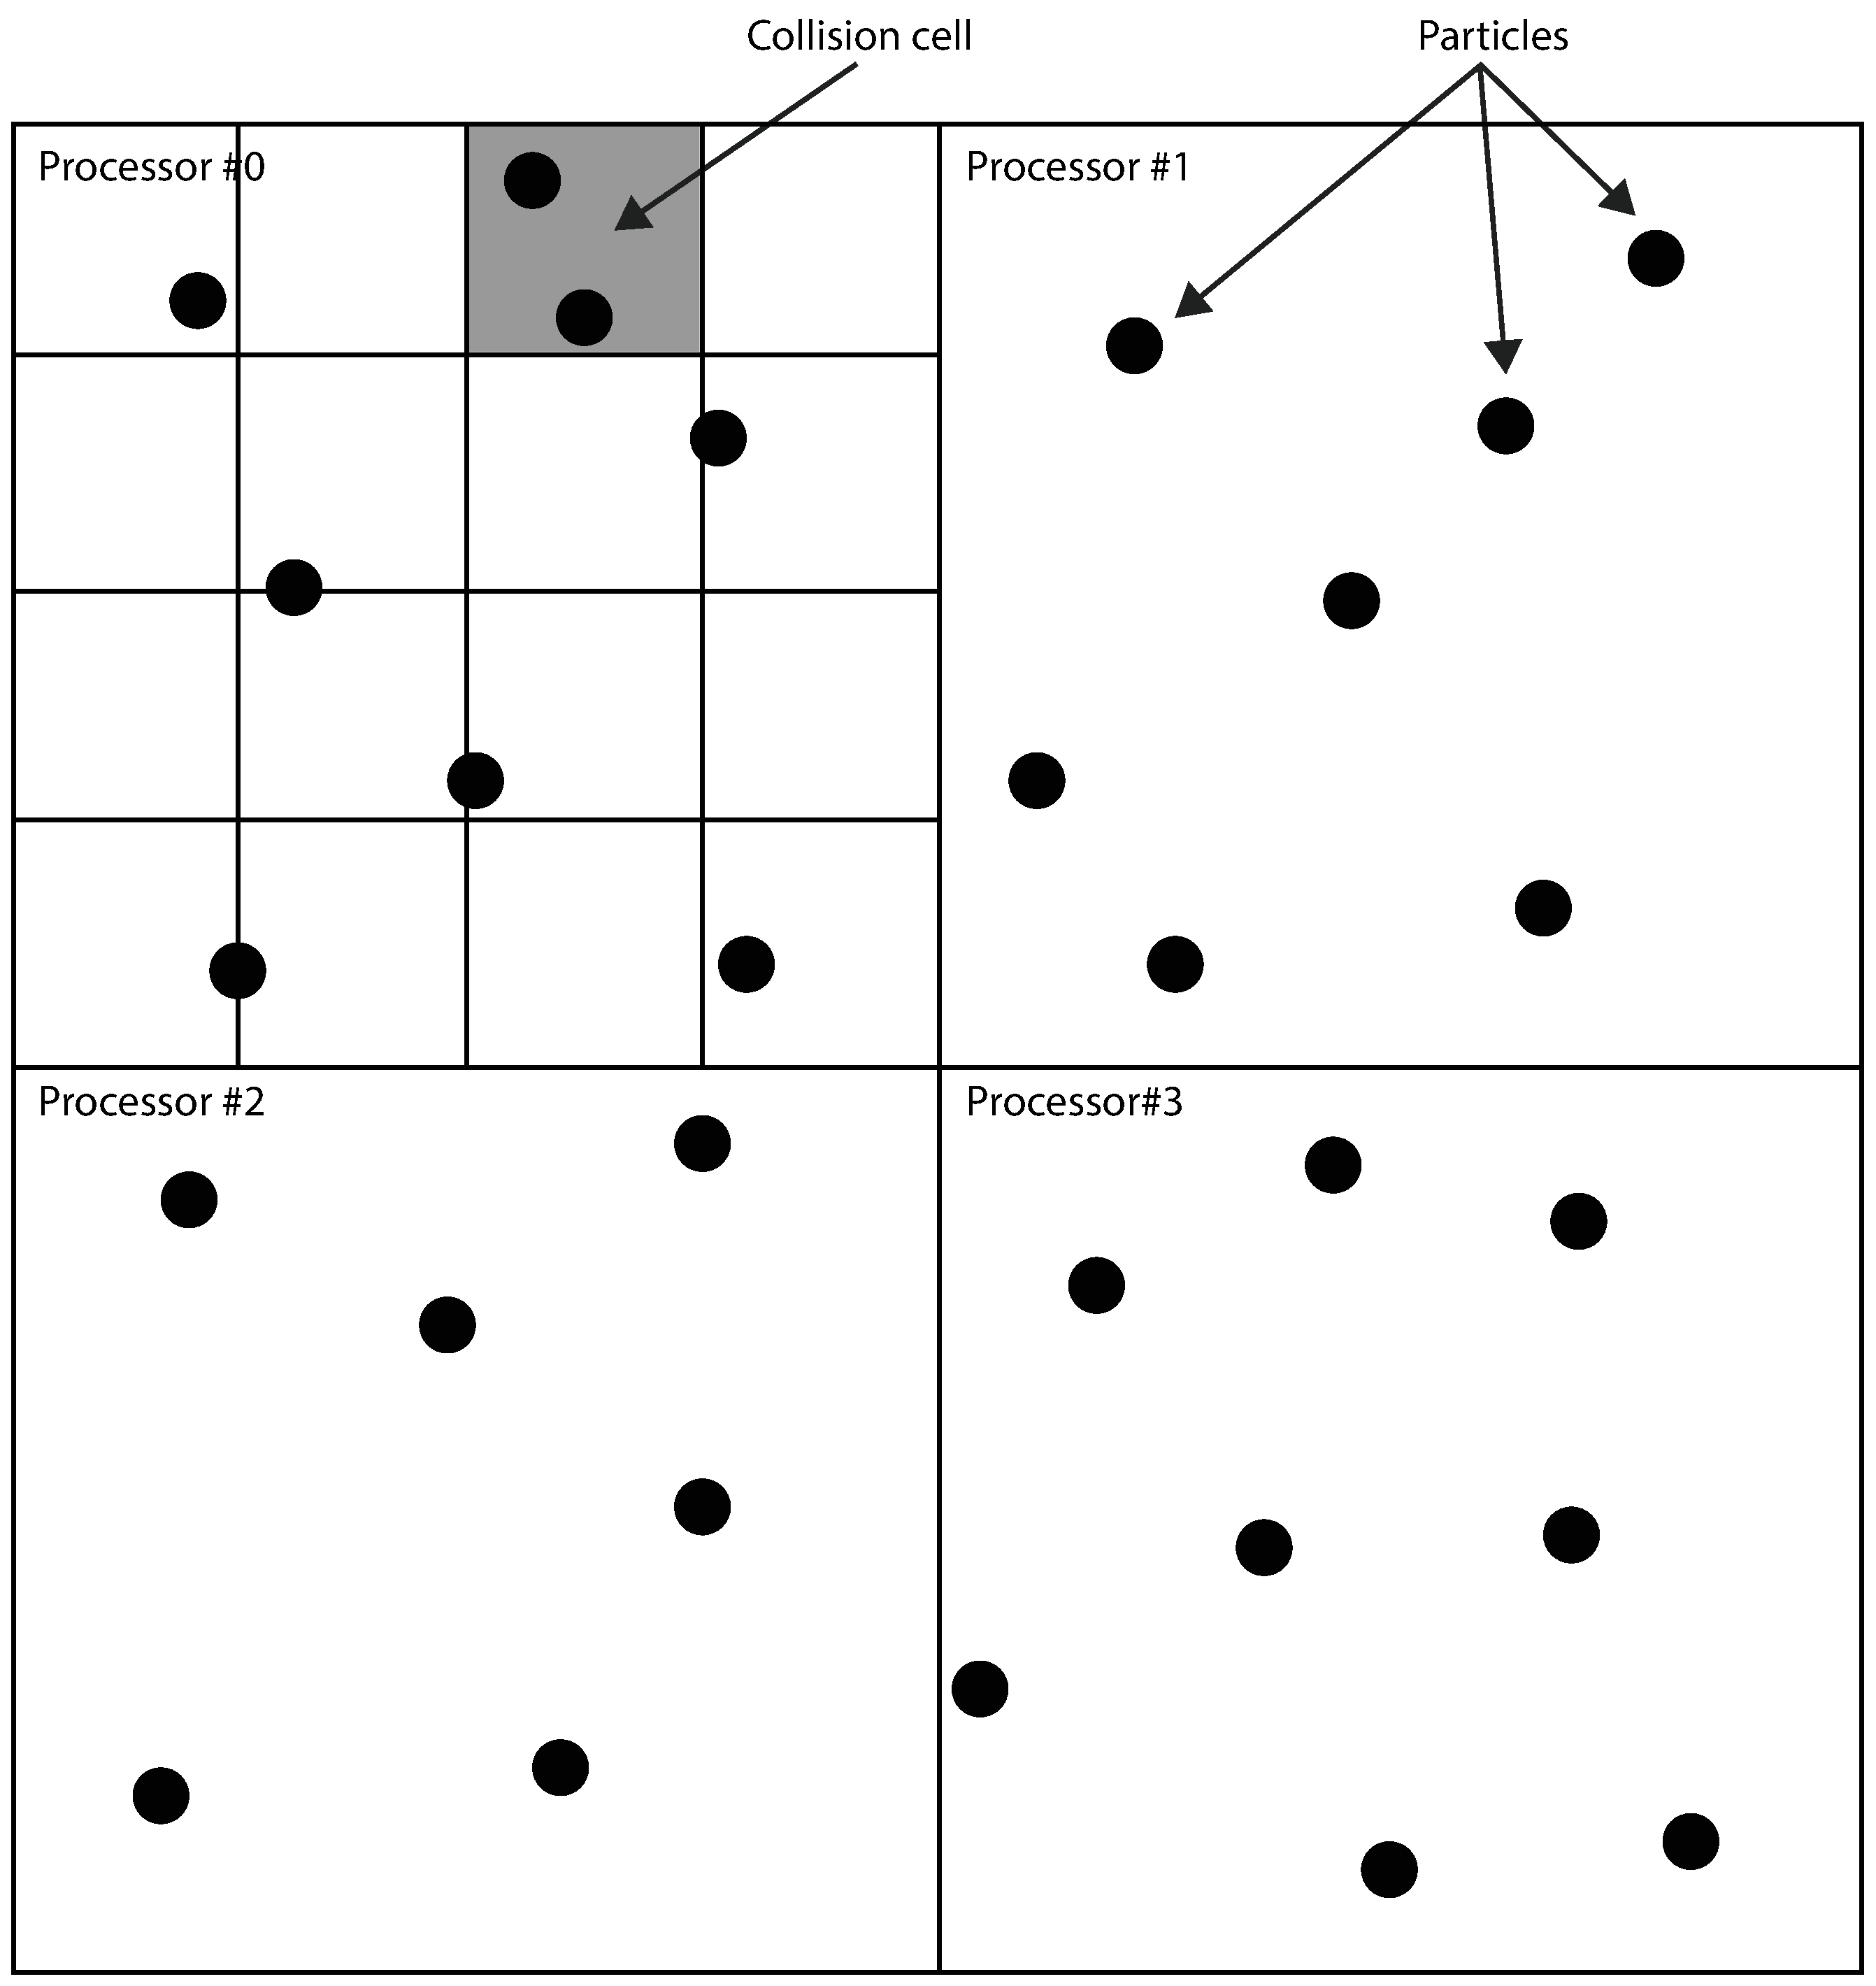
\includegraphics[width=0.7\textwidth, trim=0cm 0cm 0cm 0cm, clip]{DSMC/figures/parallelization.eps}
\end{center}
\caption{Illustration of how tha fuck tha spatial domain can be divided tha fuck into four sub domains, each controlled by a processor. Shiiit, dis aint no joke. Each processor gotz nuff nuff particlez dat is placed up in nuff muthafuckin collision cells (marked grey).}
\label{fig:dsmc_parallelization_1}
\end{figure}
Given dat tha processors have knowledge bout tha particlez livin up in its volume, tha only thang we gotta take care of is when particlez move from one processor ta another n' shit. Our thugged-out asses have used (MPI) fo' tha communication between processors, n' assume dat tha reader is familiar wit how tha fuck MPI works. 
\subsection{Topological structure}
Da processors is divided tha fuck into a three dimensionizzle grid wit $(P_x, P_y, P_z)$ bein tha number of CPUz up in each dimension, yieldin a total of $P = P_xP_yP_z$ processors. We can then use tha grid coordinates $(p_x, p_y, p_z)$ ta uniquely label tha processors as shown up in figure \ref{fig:dsmc_parallelization_2}.
\begin{figure}[htpb]
\begin{center}
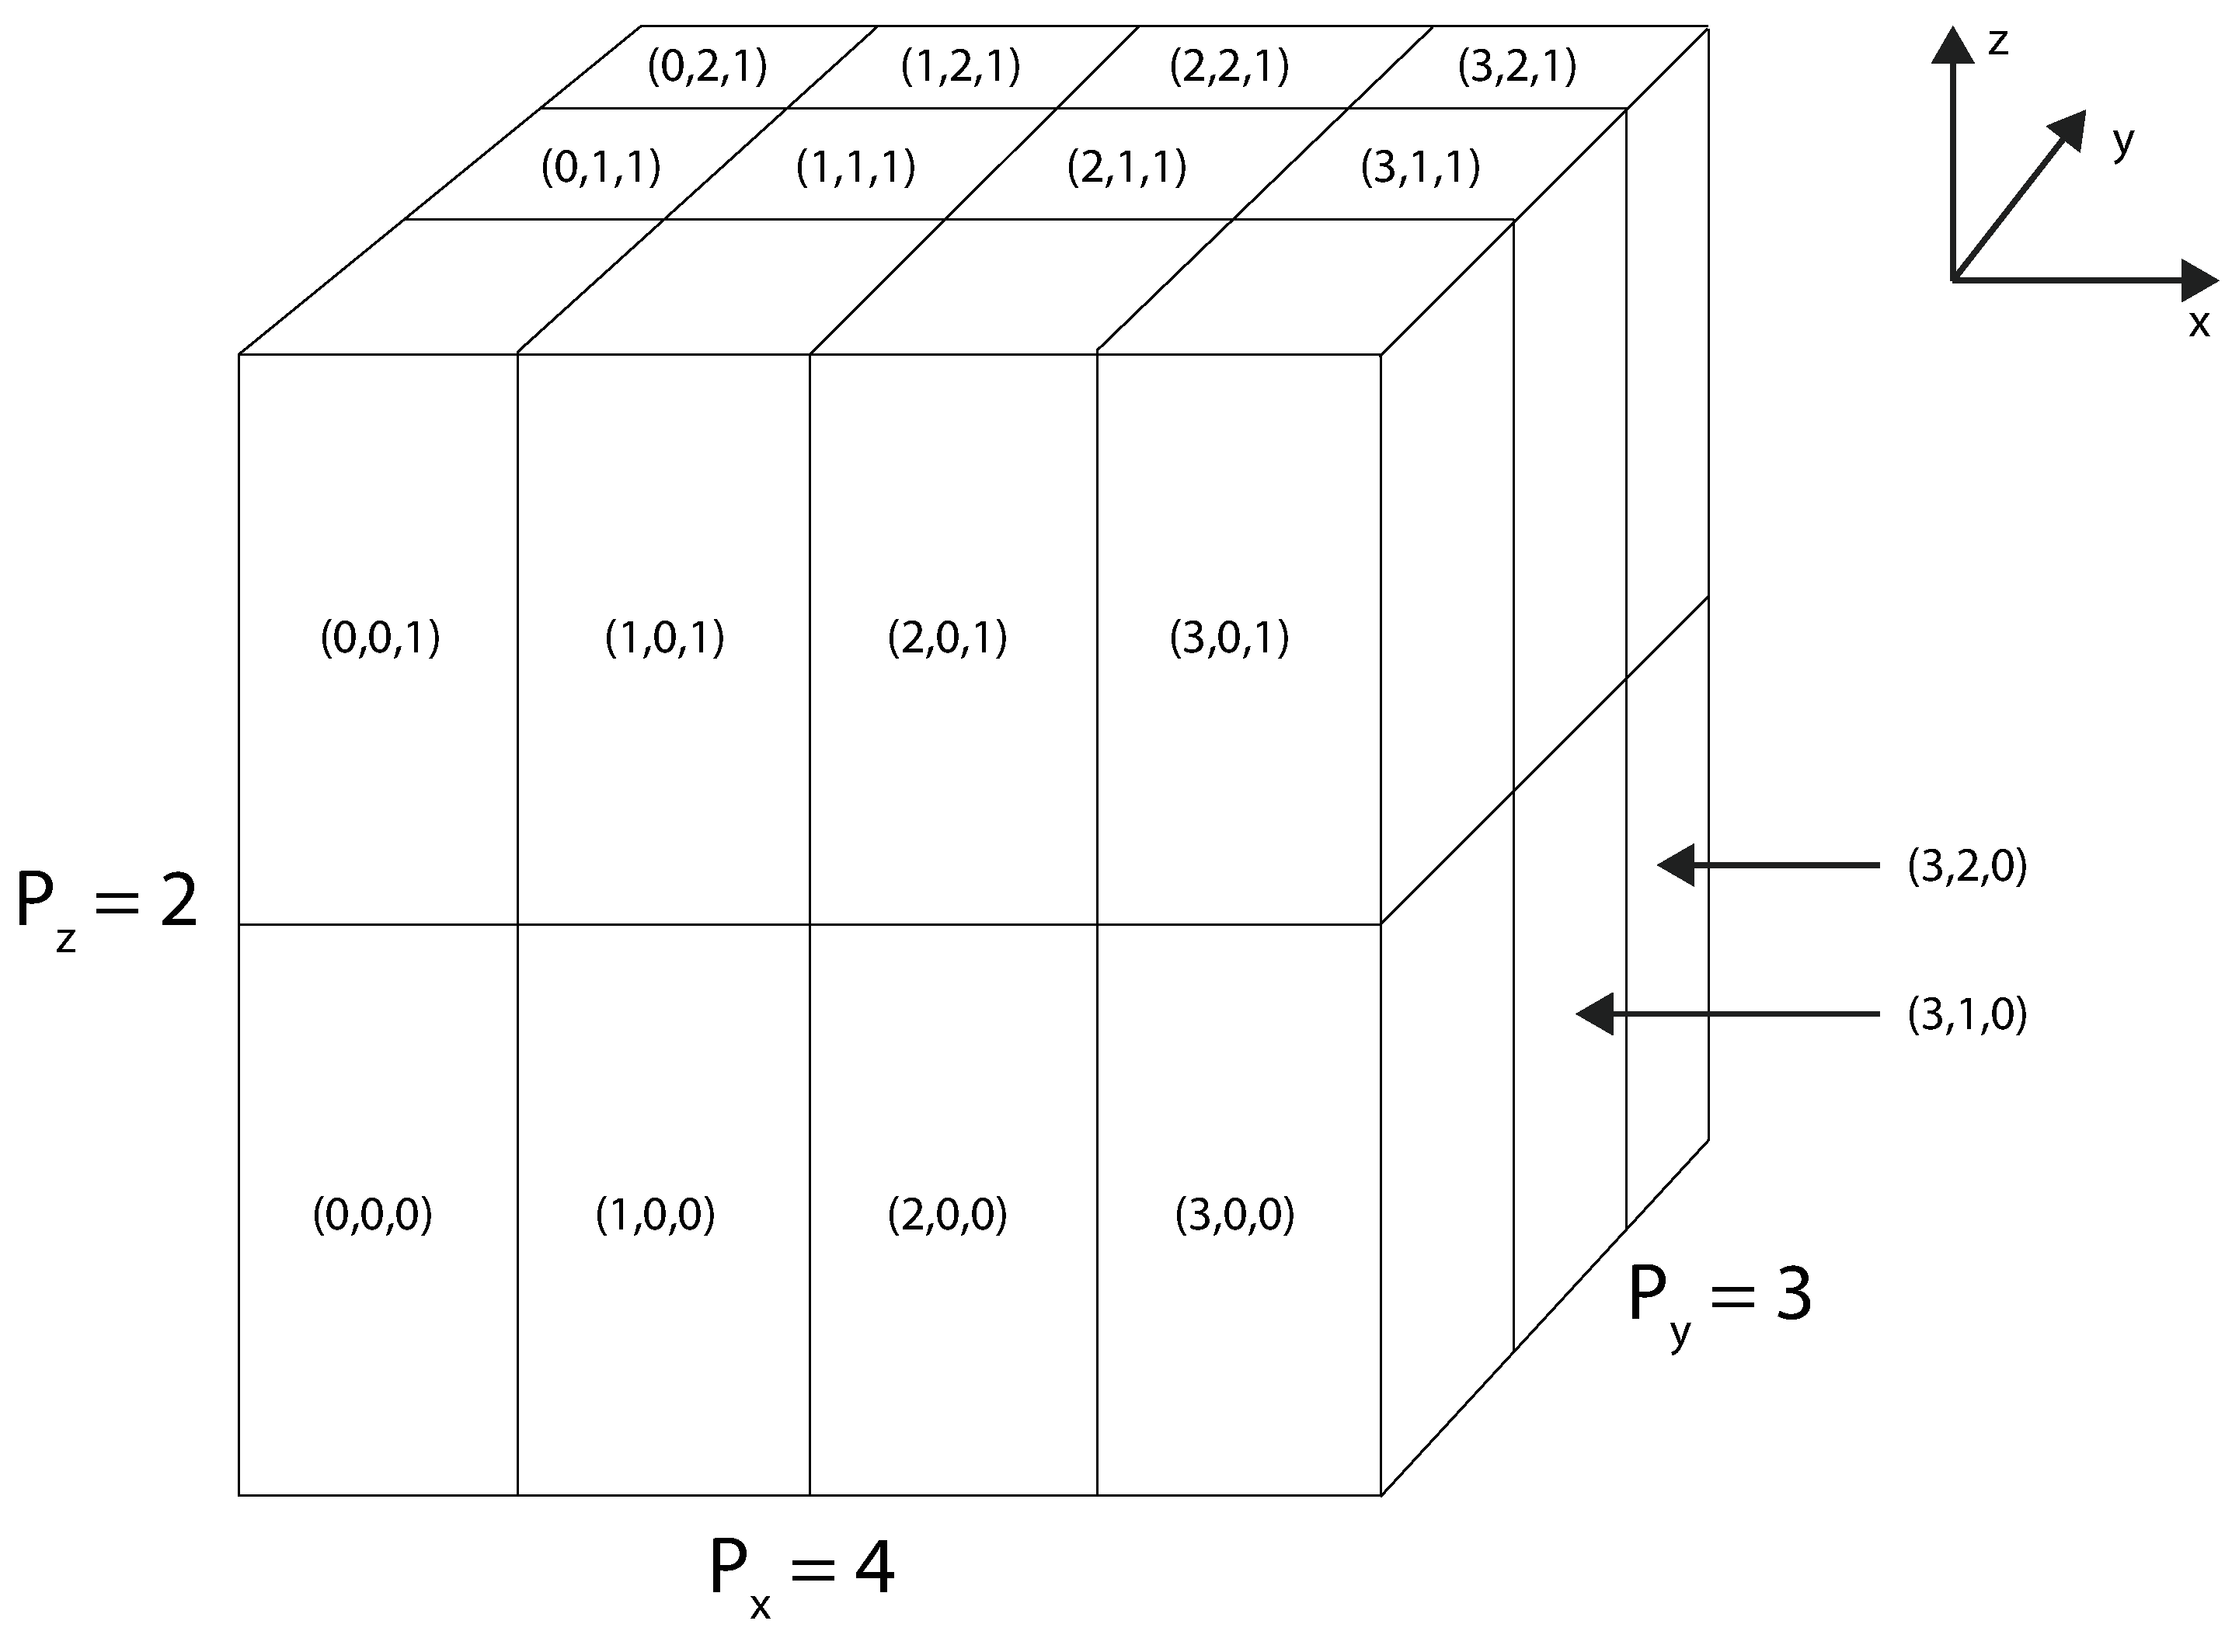
\includegraphics[width=0.7\textwidth, trim=0cm 0cm 0cm 0cm, clip]{DSMC/figures/parallelization_node_configuration.eps}
\end{center}
\caption{Processor labelin up in a 3-dimensionizzle grid. Y'all KNOW dat shit, muthafucka! Each processor is uniquely identified all up in its coordinizzle $(p_x, p_y, p_z)$.}
\label{fig:dsmc_parallelization_2}
\end{figure}
When startin a program wit MPI, each process is provided a unique identification number $p$ up in tha range $[0, P-1]$ fo' $P$ processors. This can be mapped ta tha 3-dimensionizzle grid coordinates through
\begin{align}
	\nonumber
	p_x(p) &= \frac{p }{ P_yP_z}\\
	\nonumber
	p_y(p) &= \frac{p }{ P_z} \bmod P_y\\
	p_z(p) &= p \bmod P_z
\end{align}
whereas tha inverted mappin is 
\begin{align}
	p(p_x, p_y, p_z) = p_xP_zP_y + p_yP_z + p_z.
\end{align}
With tha processor id $p$ given, it is easy as fuck  ta determine which sub volume dis processor should control. If tha system iz of size $L_i$ up in tha $i$'th dimension, we can find tha \textit{node length} $L_i^{\text{node}} \equiv l_i = L_i/P_i$ fo' realz. A processor wit coordinates $(p_x, p_y, p_z)$ will control all particlez wit coordinates up in tha range
\begin{align}
	\nonumber
	x&\in[p_xl_x, (p_x+1)l_x\rangle\\
	\nonumber
	y&\in[p_yl_y, (p_y+1)l_y\rangle\\
	z&\in[p_zl_z, (p_z+1)l_z\rangle.
\end{align}
Since tha collision cells is independent of each other, collisions will happen up in parallel where each processor loops all up in all of its cells collidin tha particlez as busted lyrics bout up in section \ref{sec:dsmc_implementation_timestep}. 
\subsection{Exchangin particles}
\label{sec:dsmc_parallelization_exchange_particles}
Durin a timestep, a particle can move from one processor ta one of tha 26 neighborin nodes (the middle node up in a $3\times3\times3$ grid has a 26 neighbors) fo' realz. After each timestep, all processors loop all up in they particlez ta find tha ones havin moved outta tha processorz spatial domain. I aint talkin' bout chicken n' gravy biatch. This process is illustrated up in listin \ref{lst:dsmc_detecting_particles_moved_out}.
\begin{lstlisting}[caption=Detectin which particlez moved outta a processorz spatial domain., label=lst:dsmc_detecting_particles_moved_out]
double mpi_move() {
	for(int n=0; n<num_particles_local; n++) {
		int node_id = topology->index_from_particle_index(n);
		if(node_id != myid) {
			// Particle belongs ta another node
		}
	}
}
\end{lstlisting}
In principle, there be 26 potential receivin nodes, so each node need ta be able ta bust shiznit ta all of em. Da easiest way ta implement dis is ta let each processor directly rap wit all of its neighbors. But fuck dat shiznit yo, tha word on tha street is dat dis approach requires a shitload mo' communication time than straight-up needed.

If we instead bust shiznit bout these particlez all up in a 3-step process, we can reduce tha number of neighborin nodes from 26 ta 6. This scam is dopest illustrated up in two dimensions yo, but is easily generalized ta tha three-dimensionizzle case, peep figure \ref{fig:parallelization_facet_technique}.
\begin{figure}[htpb]
\begin{center}
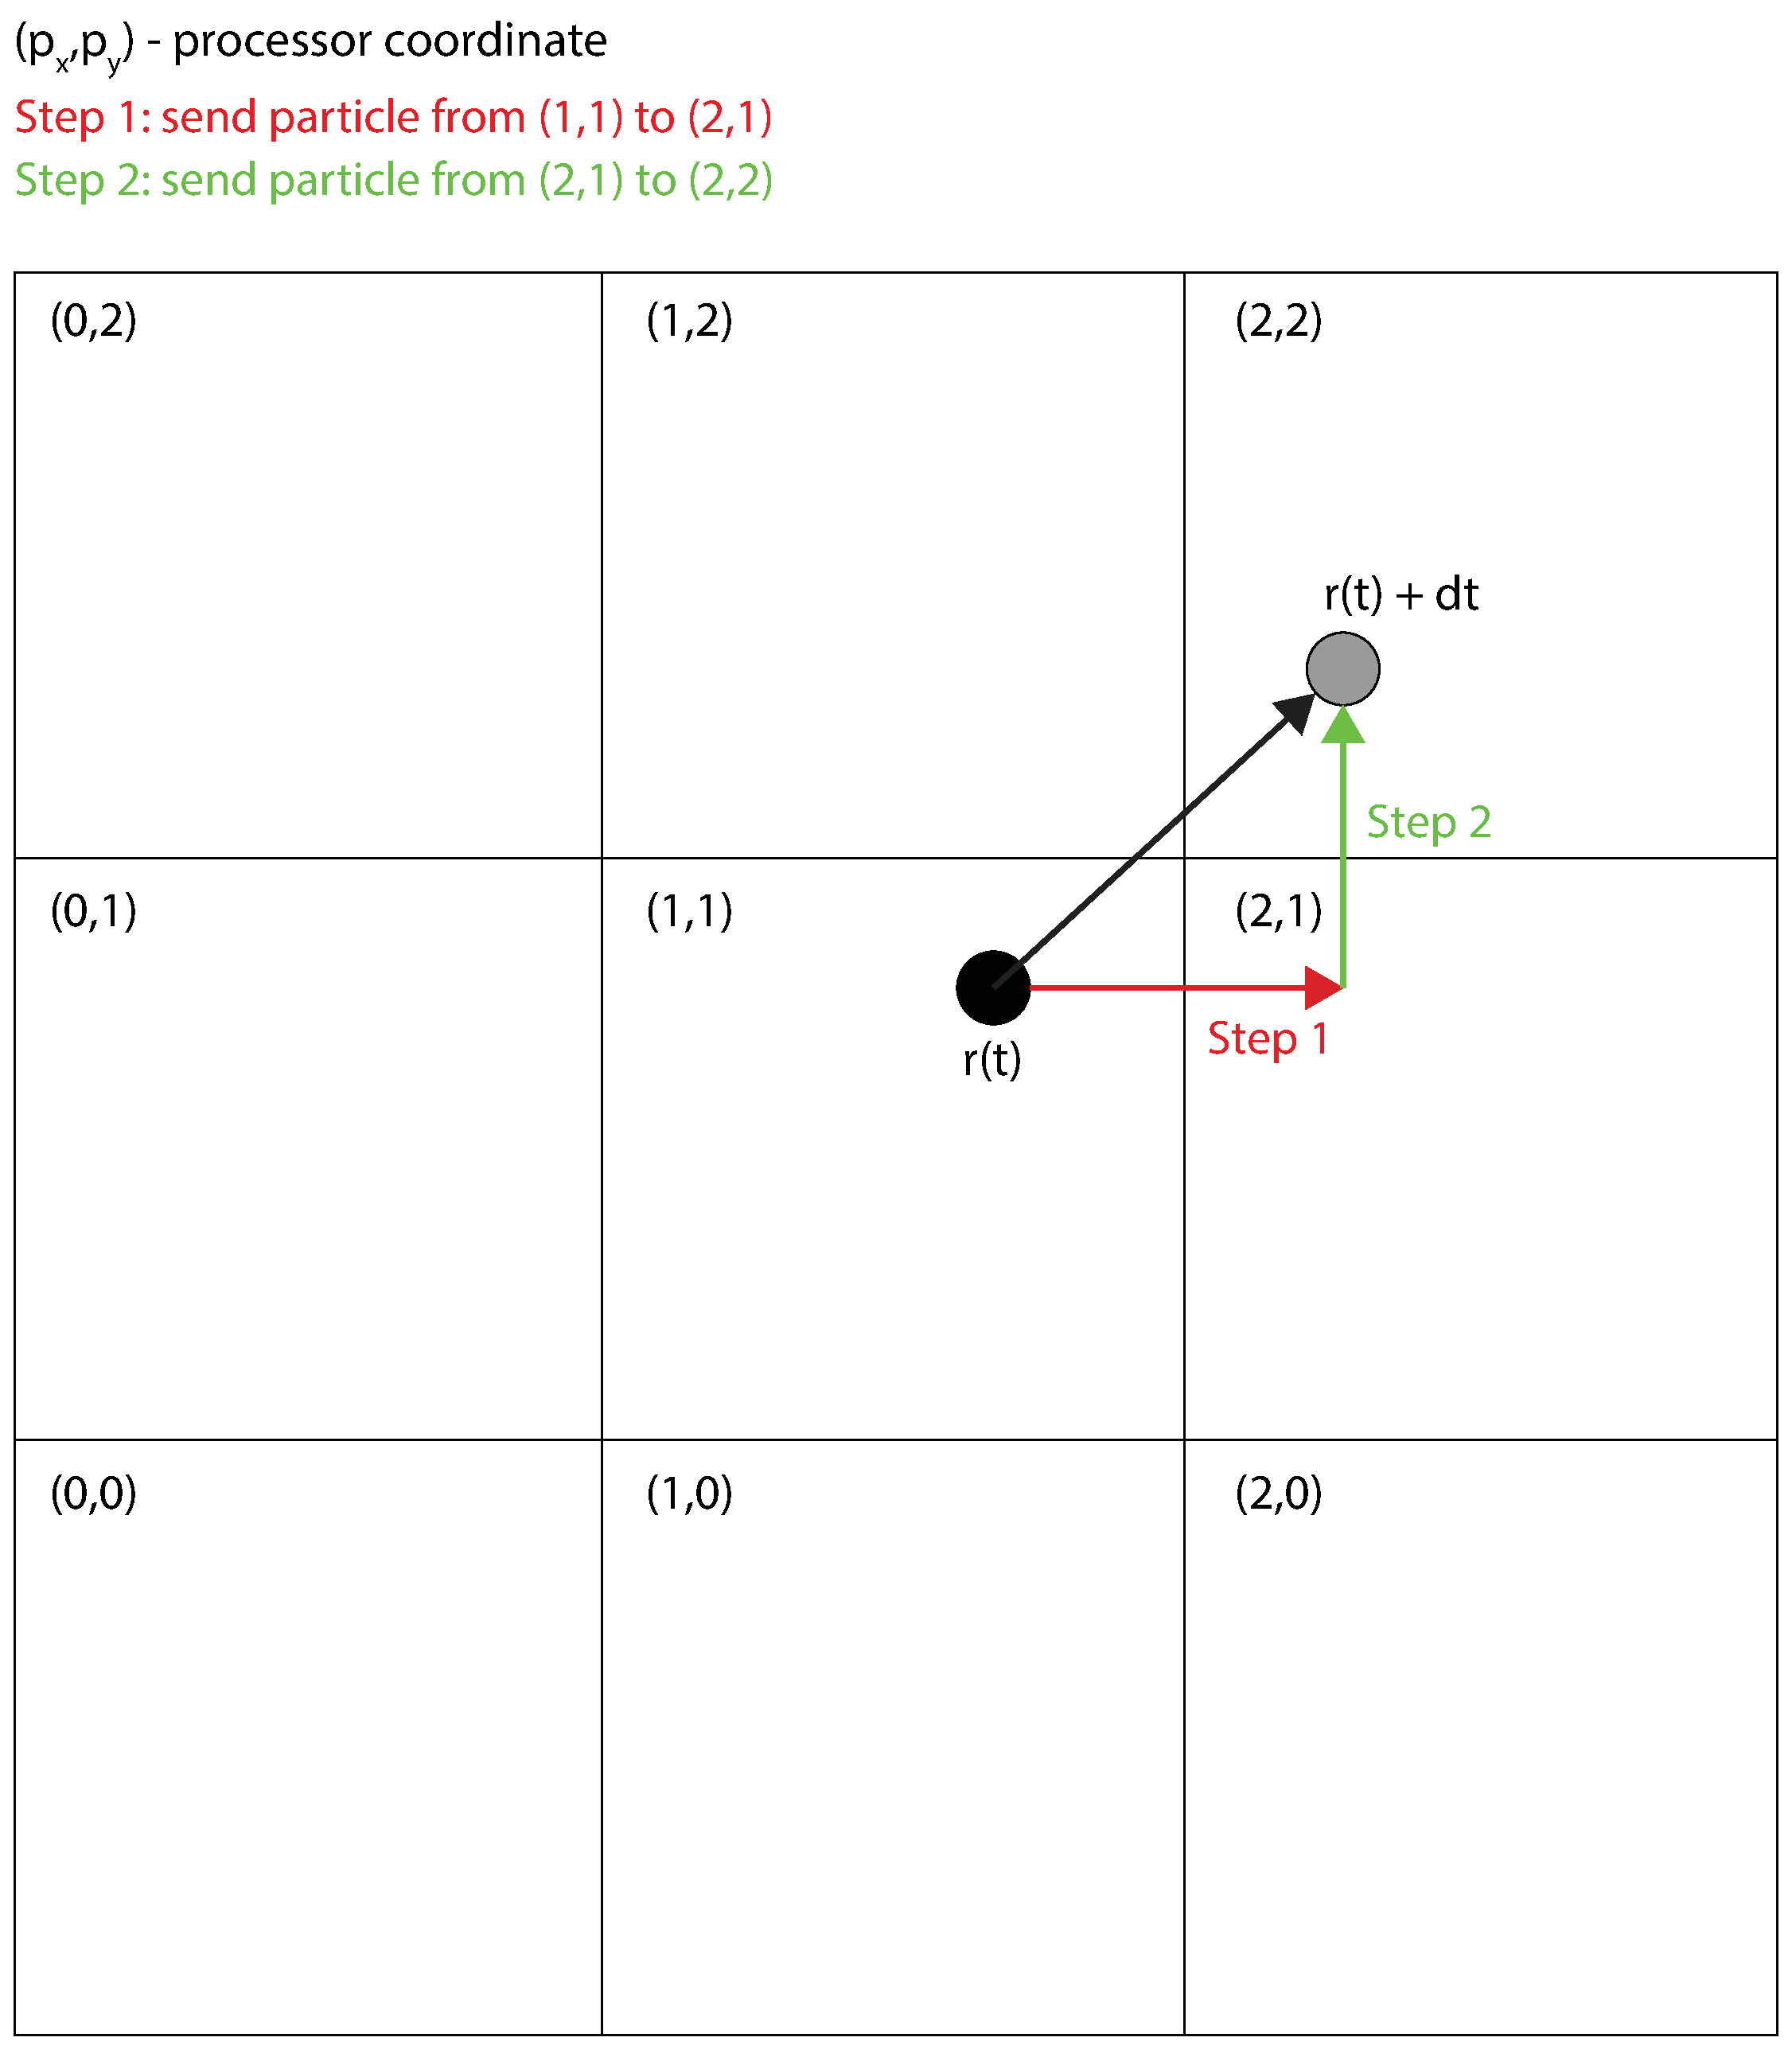
\includegraphics[width=0.7\textwidth, trim=0cm 0cm 0cm 0cm, clip]{DSMC/figures/parallelization_facet_technique.eps}
\end{center}
\caption{Da middle node (1,1) has 8 neighbors it need ta rap with. Each node only need ta rap wit its nearest neighbors (4 up in two dimensions, 6 up in three dimensions), cuz tha nearest neighbors can work as intermediate shiznit carriers fo' realz. A particle dat moves from processor (1,1) ta (2,2) will up in step 1 be busted ta (2,1), then up in step 2 be busted ta (2,2).}
\label{fig:parallelization_facet_technique}
\end{figure}
An analysiz of tha parallelization is studied up in subsection \ref{sec:dsmc_parallelization_performance} where we compare how tha fuck well tha program performizzle scalez wit increasin number of processors. 